% Options for packages loaded elsewhere
\PassOptionsToPackage{unicode}{hyperref}
\PassOptionsToPackage{hyphens}{url}
%
\documentclass[
]{article}
\title{Exploratory\_Analysis}
\author{Connie Xu}
\date{11/06/2021}

\usepackage{amsmath,amssymb}
\usepackage{lmodern}
\usepackage{iftex}
\ifPDFTeX
  \usepackage[T1]{fontenc}
  \usepackage[utf8]{inputenc}
  \usepackage{textcomp} % provide euro and other symbols
\else % if luatex or xetex
  \usepackage{unicode-math}
  \defaultfontfeatures{Scale=MatchLowercase}
  \defaultfontfeatures[\rmfamily]{Ligatures=TeX,Scale=1}
\fi
% Use upquote if available, for straight quotes in verbatim environments
\IfFileExists{upquote.sty}{\usepackage{upquote}}{}
\IfFileExists{microtype.sty}{% use microtype if available
  \usepackage[]{microtype}
  \UseMicrotypeSet[protrusion]{basicmath} % disable protrusion for tt fonts
}{}
\makeatletter
\@ifundefined{KOMAClassName}{% if non-KOMA class
  \IfFileExists{parskip.sty}{%
    \usepackage{parskip}
  }{% else
    \setlength{\parindent}{0pt}
    \setlength{\parskip}{6pt plus 2pt minus 1pt}}
}{% if KOMA class
  \KOMAoptions{parskip=half}}
\makeatother
\usepackage{xcolor}
\IfFileExists{xurl.sty}{\usepackage{xurl}}{} % add URL line breaks if available
\IfFileExists{bookmark.sty}{\usepackage{bookmark}}{\usepackage{hyperref}}
\hypersetup{
  pdftitle={Exploratory\_Analysis},
  pdfauthor={Connie Xu},
  hidelinks,
  pdfcreator={LaTeX via pandoc}}
\urlstyle{same} % disable monospaced font for URLs
\usepackage[margin=1in]{geometry}
\usepackage{longtable,booktabs,array}
\usepackage{calc} % for calculating minipage widths
% Correct order of tables after \paragraph or \subparagraph
\usepackage{etoolbox}
\makeatletter
\patchcmd\longtable{\par}{\if@noskipsec\mbox{}\fi\par}{}{}
\makeatother
% Allow footnotes in longtable head/foot
\IfFileExists{footnotehyper.sty}{\usepackage{footnotehyper}}{\usepackage{footnote}}
\makesavenoteenv{longtable}
\usepackage{graphicx}
\makeatletter
\def\maxwidth{\ifdim\Gin@nat@width>\linewidth\linewidth\else\Gin@nat@width\fi}
\def\maxheight{\ifdim\Gin@nat@height>\textheight\textheight\else\Gin@nat@height\fi}
\makeatother
% Scale images if necessary, so that they will not overflow the page
% margins by default, and it is still possible to overwrite the defaults
% using explicit options in \includegraphics[width, height, ...]{}
\setkeys{Gin}{width=\maxwidth,height=\maxheight,keepaspectratio}
% Set default figure placement to htbp
\makeatletter
\def\fps@figure{htbp}
\makeatother
\setlength{\emergencystretch}{3em} % prevent overfull lines
\providecommand{\tightlist}{%
  \setlength{\itemsep}{0pt}\setlength{\parskip}{0pt}}
\setcounter{secnumdepth}{-\maxdimen} % remove section numbering
\usepackage{booktabs}
\usepackage{longtable}
\usepackage{array}
\usepackage{multirow}
\usepackage{wrapfig}
\usepackage{float}
\usepackage{colortbl}
\usepackage{pdflscape}
\usepackage{tabu}
\usepackage{threeparttable}
\usepackage{threeparttablex}
\usepackage[normalem]{ulem}
\usepackage{makecell}
\usepackage{xcolor}
\ifLuaTeX
  \usepackage{selnolig}  % disable illegal ligatures
\fi

\begin{document}
\maketitle

\hypertarget{initial-results}{%
\subsection{Initial Results}\label{initial-results}}

First, I will be looking into the differential wage over time, in
comparison to factors such as Marital Status, Number of Biological
Children, and the availability of informal and formal childcare systems.
These findings are meant to mimic the findings of Budig and England
{[}1{]} and serve as a \textbf{very basic} starting point for testing my
hypotheses. Note that current results were adapted from work completed
in Time Series Labs using the data that I downloaded, cleaned, and
processed.

Currently, my selected dataset is the \textbf{NLSY97}. The following are
some relevant columns in the data set (as I am still trying to figure
out how to use them).

\emph{Let me know if there are better datasets out there that I can
still work with.}

\hypertarget{data-columns---values}{%
\subsection{Data Columns - Values}\label{data-columns---values}}

\begin{longtable}[]{@{}
  >{\raggedright\arraybackslash}p{(\columnwidth - 4\tabcolsep) * \real{0.21}}
  >{\raggedright\arraybackslash}p{(\columnwidth - 4\tabcolsep) * \real{0.46}}
  >{\raggedright\arraybackslash}p{(\columnwidth - 4\tabcolsep) * \real{0.32}}@{}}
\toprule
\begin{minipage}[b]{\linewidth}\raggedright
ColName
\end{minipage} & \begin{minipage}[b]{\linewidth}\raggedright
Description
\end{minipage} & \begin{minipage}[b]{\linewidth}\raggedright
Values
\end{minipage} \\
\midrule
\endhead
PUBID\_1997 & Unique Identifier & 1-8000+ \\
P2.012\_000002 & Race (Detailed) & Refer to Codebook \\
YINC.1400 & Any Income Earned this year? (Binary) & 0-1 \\
YINC.1700 & Income (Continuous) & 0-999999+ \\
KEY\_BDATE\_Y\_1997 & Birthday & 1990 - 1984 \\
CV\_HGC\_EVER\_EDT & Highest Degree Attained & 1-20, 95 = NA \\
YCCAL-1100A. 01\textasciitilde000001 & Partner Care - partner looks
after your child/children & 0-1 Variable \\
YCCAL-1100A. 01\textasciitilde000002 & Relative Care - another relative
looks after your child/children & 0-1 Variable \\
YCCAL-1100A. 02\textasciitilde000007 & Child Care Center - your child
attends a regular pre-school, Headstart, Montessori, day-care center, or
other pre-kindergarten program & 0-1 Variable \\
CV\_BIO\_CHILD\_HH & Number of Biological Children in Household & 0-5 \\
CV\_BIO\_CHILD\_NR & Number of Biological Children Outside of the House
& 0-5 \\
MAR\_STATUS.12\_XRND & Are you married as of December & 0.0 - Never
Married Not Cohabitating, 1.0 - Never Married Cohabiting, 2.0 - Married,
3.0 - Legally Separated, 4.0 - Divorced, 5.0 - Widowed \\
\bottomrule
\end{longtable}

These are some summary statistics that I have identified thus far with
panel data. As we can see, when I filter for years in which the
individual(s) have children and / or valid income data (I imputed some
missing values as well) our range is from 1998 - 2017 (nearly 20 years
in range).

\textbf{Table 1}

\begin{tabular}{l|r|r|r|r|r|r|r|r|r|r|r|r|r}
\hline
  & vars & n & mean & sd & median & trimmed & mad & min & max & range & skew & kurtosis & se\\
\hline
PUBID\_1997 & 1 & 63436 & 4.622395e+03 & 2.593539e+03 & 4699 & 4.644521e+03 & 3276.5460 & 1 & 9022 & 9021 & -0.0645019 & -1.1733818 & 10.2973357\\
\hline
year & 2 & 63436 & 2.006126e+03 & 5.447551e+00 & 2006 & 2.005853e+03 & 5.9304 & 1998 & 2017 & 19 & 0.3201443 & -0.8768813 & 0.0216288\\
\hline
MARRIED\_OR\_COHABITATING & 3 & 63043 & 3.754422e-01 & 4.842407e-01 & 0 & 3.443046e-01 & 0.0000 & 0 & 1 & 1 & 0.5144378 & -1.7353813 & 0.0019286\\
\hline
INCOME & 4 & 54466 & 1.402693e+04 & 2.029355e+04 & 5000 & 1.012587e+04 & 7413.0000 & 0 & 235884 & 235884 & 3.0159561 & 17.6265351 & 86.9551308\\
\hline
N\_CHILDREN & 5 & 63436 & 7.471783e-01 & 1.105296e+00 & 0 & 5.302266e-01 & 0.0000 & 0 & 8 & 8 & 1.5821394 & 2.4335302 & 0.0043884\\
\hline
INTERGENERATION\_CHILDCARE & 6 & 63436 & 1.228010e-02 & 1.101339e-01 & 0 & 0.000000e+00 & 0.0000 & 0 & 1 & 1 & 8.8567110 & 76.4425340 & 0.0004373\\
\hline
SPOUSAL\_CHILDCARE & 7 & 63436 & 6.447400e-03 & 8.003730e-02 & 0 & 0.000000e+00 & 0.0000 & 0 & 1 & 1 & 12.3328642 & 150.1019067 & 0.0003178\\
\hline
CHILDCARE\_CENTER & 8 & 63436 & 1.797100e-03 & 4.235430e-02 & 0 & 0.000000e+00 & 0.0000 & 0 & 1 & 1 & 23.5251305 & 551.4404600 & 0.0001682\\
\hline
CV\_HGC\_EVER\_EDT & 9 & 63436 & 1.271478e+01 & 2.795374e+00 & 12 & 1.263109e+01 & 2.9652 & 5 & 20 & 15 & 0.3016162 & -0.2711200 & 0.0110987\\
\hline
\end{tabular}

As shown below, it is clear that there are differences between income
trajectories over time for women with children and women without (on
average).

\textbf{Figure 1: Mean Income Over Time}
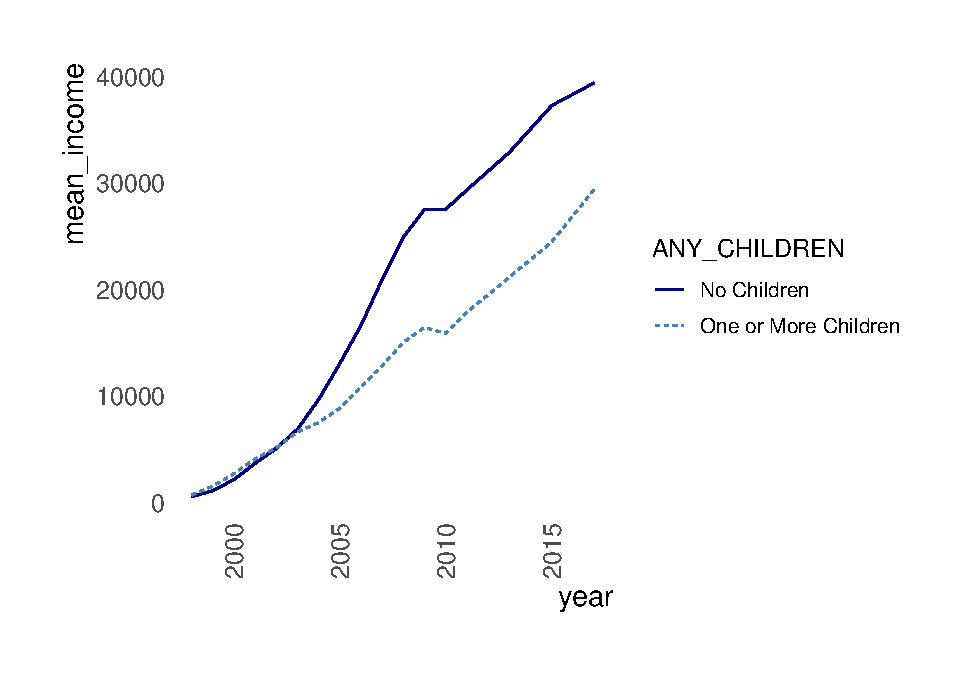
\includegraphics{Exploratory_Analysis_files/figure-latex/Figure 1-1.pdf}
\#\# Basic Models

\begin{verbatim}
% Table created by stargazer v.5.2.2 by Marek Hlavac, Harvard University. E-mail: hlavac at fas.harvard.edu
% Date and time: Thu, Nov 18, 2021 - 13:04:27
% Requires LaTeX packages: dcolumn 
\begin{table}[!htbp] \centering 
  \caption{Regression Results} 
  \label{} 
\begin{tabular}{@{\extracolsep{5pt}}lD{.}{.}{-3} D{.}{.}{-3} D{.}{.}{-3} } 
\\[-1.8ex]\hline 
\hline \\[-1.8ex] 
\\[-1.8ex] & \multicolumn{3}{c}{Income} \\ 
\\[-1.8ex] & \multicolumn{1}{c}{\textit{OLS}} & \multicolumn{2}{c}{\textit{panel}} \\ 
 & \multicolumn{1}{c}{\textit{}} & \multicolumn{2}{c}{\textit{linear}} \\ 
 & \multicolumn{1}{c}{Pooled} & \multicolumn{1}{c}{First Diff} & \multicolumn{1}{c}{Fixed Effects} \\ 
\hline \\[-1.8ex] 
 Children & -4,324.656^{***} & -1,709.998^{***} & -4,038.936^{***} \\ 
  & (74.212) & (130.652) & (102.549) \\ 
  1999 & 747.561^{*} & 758.166^{***} & 675.538^{**} \\ 
  & (402.554) & (218.954) & (335.219) \\ 
  as.factor(year)2000 & 2,121.468^{***} & 2,005.616^{***} & 1,875.135^{***} \\ 
  & (409.329) & (305.499) & (341.714) \\ 
  as.factor(year)2001 & 3,943.418^{***} & 3,752.590^{***} & 3,813.738^{***} \\ 
  & (407.381) & (372.732) & (340.426) \\ 
  as.factor(year)2002 & 5,667.058^{***} & 5,420.105^{***} & 5,485.868^{***} \\ 
  & (419.781) & (436.623) & (351.706) \\ 
  as.factor(year)2003 & 7,939.058^{***} & 7,238.291^{***} & 7,551.947^{***} \\ 
  & (421.070) & (488.542) & (353.532) \\ 
  as.factor(year)2004 & 10,466.500^{***} & 9,381.513^{***} & 9,796.622^{***} \\ 
  & (425.140) & (536.620) & (357.910) \\ 
  as.factor(year)2005 & 13,390.250^{***} & 12,034.150^{***} & 12,825.620^{***} \\ 
  & (427.747) & (583.100) & (361.251) \\ 
  as.factor(year)2006 & 16,558.640^{***} & 14,600.850^{***} & 15,729.910^{***} \\ 
  & (423.454) & (627.129) & (358.428) \\ 
  as.factor(year)2007 & 19,921.270^{***} & 17,875.150^{***} & 19,199.960^{***} \\ 
  & (425.720) & (675.016) & (361.685) \\ 
  as.factor(year)2008 & 23,155.170^{***} & 20,558.740^{***} & 22,409.420^{***} \\ 
  & (419.441) & (722.707) & (357.763) \\ 
  as.factor(year)2009 & 25,215.760^{***} & 22,272.410^{***} & 24,527.590^{***} \\ 
  & (414.564) & (779.502) & (354.850) \\ 
  as.factor(year)2010 & 24,912.740^{***} & 21,887.520^{***} & 24,371.980^{***} \\ 
  & (417.415) & (842.153) & (359.126) \\ 
  as.factor(year)2011 & 26,875.050^{***} & 23,560.720^{***} & 26,351.530^{***} \\ 
  & (417.391) & (908.075) & (360.816) \\ 
  as.factor(year)2013 & 30,338.240^{***} & 26,661.140^{***} & 29,832.040^{***} \\ 
  & (424.479) & (977.432) & (370.633) \\ 
  as.factor(year)2015 & 34,101.870^{***} & 29,786.000^{***} & 33,476.800^{***} \\ 
  & (430.252) & (1,051.060) & (378.965) \\ 
  as.factor(year)2017 & 38,391.440^{***} & 33,963.420^{***} & 37,820.860^{***} \\ 
  & (431.546) & (1,135.408) & (383.275) \\ 
 \hline \\[-1.8ex] 
Observations & \multicolumn{1}{c}{54,466} & \multicolumn{1}{c}{50,150} & \multicolumn{1}{c}{54,466} \\ 
R$^{2}$ & \multicolumn{1}{c}{0.282} & \multicolumn{1}{c}{0.030} & \multicolumn{1}{c}{0.346} \\ 
Adjusted R$^{2}$ & \multicolumn{1}{c}{0.282} & \multicolumn{1}{c}{0.030} & \multicolumn{1}{c}{0.289} \\ 
Residual Std. Error & \multicolumn{1}{c}{17,198.880 (df = 54448)} &  &  \\ 
F Statistic & \multicolumn{1}{c}{1,257.682$^{***}$ (df = 17; 54448)} & \multicolumn{1}{c}{92.683$^{***}$ (df = 17; 50132)} & \multicolumn{1}{c}{1,557.435$^{***}$ (df = 17; 50133)} \\ 
\hline 
\hline \\[-1.8ex] 
\textit{Note:}  & \multicolumn{3}{r}{$^{*}$p$<$0.1; $^{**}$p$<$0.05; $^{***}$p$<$0.01} \\ 
\end{tabular} 
\end{table} 
\end{verbatim}

\emph{Note: The `Year' coefficients correspond to distance from the base
year (1998).}

This is a simple OLS, looking at the time based values, Marital Status,
and number of biological children. The results show that the respondents
appear to increase between approx. \$900 and \$4K per year with no other
items in the model. Additionally, each additional child corresponds with
\$4K.3 less income per year for these respondents (on average across the
sampled population)

The independent variable (N\_CHILDREN) is very statistically significant
(P values are far below threshold of 0.05); thus we are able to reject
the null hypothesis (i.e., that the predictor or independent variable
doesn't have a significant relationship with the dependent variable).

Also note that the R-Squared is 0.34, which indicates an approximate
34\% explained variance by our coefficients (time and number of
children) - I think this makes sense because a lot of income is a
function simply of time at work / accumulation of human capital (see
Figure 1 above).

This is obviously a very basic model, as we don't control for basic
aspects of human capital such as education level (but we will so in
better models later in this lab).

\hypertarget{first-differences}{%
\subsubsection{First Differences}\label{first-differences}}

Here, we are able to see that the influence of number of children that
individuals have continues to be important; here we are only building
model with non unique observations (54466-4316). Note that first
difference uses panel data to control for individual heterogeneity.

The results are consistent with existing literature and with previous
findings in the pooled OLS model. For each additional child that a woman
has, annual income decreases by \$1.7K on average (for the same person
across the 9 years of data net of year/wave of survey). We can also see
that \textbf{statistical significance of the model doesn't appear to
change} as p-value continues to be very small (well below 0.05) allowing
us to reject the null that there is no relationship. Note also however
the very \textbf{low R-Squared} in this model, showing that using first
differences, the variable of number of children only explains 3\% of
variance in our dependent variable.

When using the fixed effects model, our findings are consistent once
more with the previous models. For each additional child that women have
from before (i.e., change in number of children), income decreases by
\$4K on average, net of difference across individual persons across
1998-2017 panels. This finding is \textbf{statistically significant,
with a p-value well below 0.05} at 2.22e-16; further, this model, which
looks at \emph{within} transformations using individual `demeaned
effects' (i.e., we are comparing effects from the individual's mean
rather than comparing between waves of data), appears once more to be
more explanatory (i.e., \textbf{adjusted r-squared of 0.29}) relative to
the first difference model. Based on these methods, the degree of
variation and overall nature of the dependent variable would differ
between First Differencing and Fixed Effects, which would naturally
impact the \textbf{proportion of explained variance}

\hypertarget{initial-models-with-control-variables}{%
\subsection{Initial Models (with Control
Variables)}\label{initial-models-with-control-variables}}

This time, I wanted to control for other human capital factors, such as
Education Level and Marital Status. \emph{I tried to interpret with an
interaction term - please correct if the interaction portion is
inaccurate. If you want to look at the simpler model without
interactions, please refer to my third model.}

\begin{verbatim}
Regression Results - With Control Variables
=======================================================================================================
                                                                  Income                               
                                   Fixed Effects: Interaction Terms Fixed Effects: No Interaction Terms
-------------------------------------------------------------------------------------------------------
Children                                     2,139.539***                      2,145.181***            
                                               (52.656)                          (52.698)              
1999                                        -2,365.083***                      -3,244.332***           
                                              (140.381)                          (104.377)             
MARRIED_OR_COHABITATING                      4,419.658***                      3,308.538***            
                                              (209.671)                          (172.948)             
as.factor(year)1999                         -1,203.148***                      -1,165.895***           
                                              (331.590)                          (331.854)             
as.factor(year)2000                         -1,943.494***                      -1,838.124***           
                                              (345.656)                          (345.772)             
as.factor(year)2001                         -1,772.823***                      -1,594.398***           
                                              (355.640)                          (355.436)             
as.factor(year)2002                         -1,602.101***                      -1,360.687***           
                                              (378.130)                          (377.576)             
as.factor(year)2003                           -811.640**                         -511.732              
                                              (391.607)                          (390.632)             
as.factor(year)2004                            387.649                           748.206*              
                                              (405.437)                          (403.952)             
as.factor(year)2005                          2,634.818***                      3,064.364***            
                                              (417.133)                          (414.959)             
as.factor(year)2006                          4,837.819***                      5,307.160***            
                                              (422.046)                          (419.418)             
as.factor(year)2007                          7,740.750***                      8,234.630***            
                                              (431.488)                          (428.619)             
as.factor(year)2008                         10,487.720***                      11,010.070***           
                                              (434.359)                          (431.130)             
as.factor(year)2009                         12,276.900***                      12,809.980***           
                                              (436.154)                          (432.792)             
as.factor(year)2010                         11,755.690***                      12,314.880***           
                                              (444.719)                          (441.068)             
as.factor(year)2011                         13,458.040***                      14,003.080***           
                                              (451.021)                          (447.631)             
as.factor(year)2013                         16,309.770***                      16,837.090***           
                                              (465.461)                          (462.438)             
as.factor(year)2015                         19,608.760***                      20,131.410***           
                                              (478.943)                          (476.087)             
as.factor(year)2017                         23,697.440***                      24,208.410***           
                                              (487.085)                          (484.434)             
N_CHILDREN:MARRIED_OR_COHABITATING          -1,349.506***                                              
                                              (144.235)                                                
-------------------------------------------------------------------------------------------------------
Observations                                    54,130                            54,130               
R2                                              0.375                              0.374               
Adjusted R2                                     0.321                              0.320               
F Statistic                         1,494.775*** (df = 20; 49811)      1,566.119*** (df = 19; 49812)   
=======================================================================================================
Note:                                                                       *p<0.1; **p<0.05; ***p<0.01
\end{verbatim}

\hypertarget{fixed-effects-interaction-terms}{%
\subsubsection{Fixed Effects: Interaction
Terms}\label{fixed-effects-interaction-terms}}

Once more, the results are once more consistent with existing
literature. It seems that for each change (addition) in number of
children that a woman has (without changing marital status), income
decreases by \$2K on average, net of difference across individual
persons across 1998-2017 panels; net of changes in education levels.
This decrease appears to be exacerbated on average for individuals who
are married/cohabitating: women who both become married/cohabitating and
have additional children experience annual income decrease of \$1.3K
additionally on average, even as changing from unmarried to
married/cohabitating (with no change in number of children) appears to
correspond on average to additional \$4.4K increase in income - all of
this net of individual person across 1998-2017 panels and net of changes
in education level.

Additionally, it may appear that the addition of the education variable
has created interpretability difficulties in the model, as youths in the
NLSY earlier waves would be continuing school likely at the same rate as
the `year' (though this is not guranteed). However, it appears that each
additional year of education corresponds to increase of \$2.1K of income
net of time and marriage / child factors.

All of these coefficients have exhibited very high t-value and p-values;
the whole model also exhibits \textbf{a high f statistic and p-value
well below 0.05} at 2.22e-16. Finally it should be noted that this model
has the \textbf{highest r squared yet at 0.32 adjusted r-squared},
indicating that the added variables seem to be explaining more variance
to this model.

\hypertarget{fixed-effects-no-interaction-terms}{%
\subsubsection{Fixed Effects: No Interaction
Terms}\label{fixed-effects-no-interaction-terms}}

Overall, the results are once more consistent with existing literature.
For each change in number of children that women have, (without changing
marital status), income decreases by \$3.2K on average, net of
difference across individual persons across 1998-2017 panels and net of
changes in education and marital status.

Meanwhile, changing from unmarried to married corresponds with income
increase by \$3.3K on average, net of difference across individual
persons across 1998-2017 panels and net of changes in education and
number of children.

As discussed above, the addition of the education variable has created
interpretability difficulties in the model, as youths in the NLSY
earlier waves would be continuing school likely at the same rate as the
`year' (though this is not guranteed). However, it appears that each
additional year of education corresponds to increase of \$2.1K of income
net of time and marriage / child factors.

All of these coefficients have exhibited very high t-value and p-values;
the whole model also exhibits \textbf{a high f statistic and p-value
well below 0.05} at 2.22e-16. Finally it should be noted that this model
has the \textbf{highest r squared yet at 0.32 adjusted r-squared},
indicating that the added variables seem to be explaining more variance
to this model.

\begin{center}\rule{0.5\linewidth}{0.5pt}\end{center}

{[}1{]}Budig, M. J., \& England, P. (2001). The Wage Penalty for
Motherhood. American Sociological Review, 66(2), 204--225.
\url{https://doi.org/10.2307/2657415}

\end{document}
